\documentclass[tikz]{standalone}

\usepackage{graphicx}
\usepackage{tikz}
\usetikzlibrary{quotes}

\tikzstyle{every picture} = [node distance=1.3cm]


\begin{document} 
        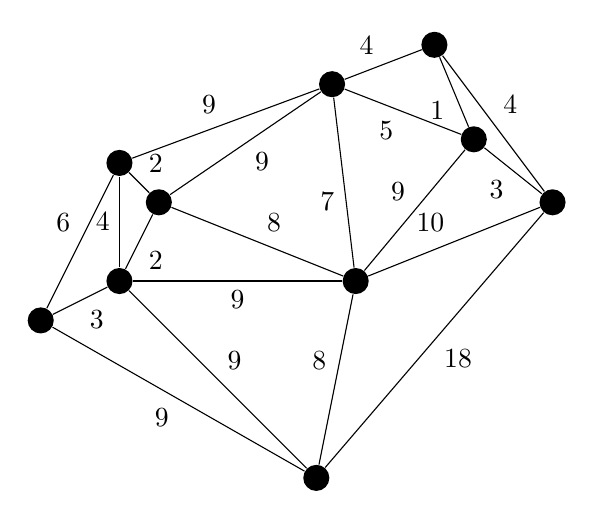
\begin{tikzpicture} 
            \node (node 1) at(0,3) [circle,double, double distance =1.2pt,text=white,fill=black,] {};
            \node (node 2) at(1,3.5) [circle,double, double distance =1.2pt,text=white,fill=black,] {};
            \node (node 3) at(1.5,4.5) [circle,double, double distance =1.2pt,text=white,fill=black,] {};
            \node (node 4) at(1,5) [circle,double, double distance =1.2pt,text=white,fill=black,] {};
            \node (node 5) at(3.5,1) [circle,double, double distance =1.2pt,text=white,fill=black,] {};
            \node (node 6) at(4,3.5) [circle,double, double distance =1.2pt,text=white,fill=black,] {};
			\node (node 7) at(3.7,6) [circle,double, double distance =1.2pt,text=white,fill=black,] {};
			\node (node 8) at(5,6.5) [circle,double, double distance =1.2pt,text=white,fill=black,] {};
			\node (node 9) at(5.5,5.3) [circle,double, double distance =1.2pt,text=white,fill=black,] {};
			\node (node 10) at(6.5,4.5) [circle,double, double distance =1.2pt,text=white,fill=black,] {};
            
            
            \path 	(node 2) edge[-,"3"] (node 1)
            		(node 4) edge[-,"2"] (node 3)
            		(node 2) edge[-,"4"] (node 4)
            		(node 1) edge[-,"6"] (node 4)
            		(node 9) edge[-,"1"] (node 8)
            		(node 9) edge[-,"5"] (node 7)
            		(node 5) edge[-,"9"] (node 1)
            		(node 8) edge[-,"4"] (node 10)
            		(node 10) edge[-,"3"] (node 9)
            		(node 6) edge[-,"9"] (node 9)
            		(node 2) edge[-,"9"] (node 5)
            		(node 6) edge[-,"9"] (node 2)
            		(node 3) edge[-,"8"] (node 6)
            		(node 7) edge[-,"9"] (node 3)
            		(node 6) edge[-,"10"] (node 10)
            		(node 4) edge[-,"9"] (node 7)
            		(node 6) edge[-,"7"] (node 7)
            		(node 5) edge[-,"8"] (node 6)
            		(node 7) edge[-,"4"] (node 8)
            		(node 10) edge[-,"18"] (node 5)
            		(node 3) edge[-,"2"] (node 2);
            	
            
                  

        \end{tikzpicture}
\end{document}